%!TEX root = ../main.tex

\section{Preliminaries}\label{sec:preliminaries}
We employ standard terminology from (finite and classical) model theory~\cite[Sec. 1--3]{Libkin04}.

All the logics considered in this paper are fragments of the first-order logic ($\FO$) over purely-relational equality-free vocabularies, under the usual syntax and semantics. 
We fix a countably infinite set $\V \deff \{x_i \colon\, i \in \N\}$ of variables and a countably infinite set~$\R$ of predicates (we employ $\arity(\relR)$ to denote the arity of $\relR$ from $\R$).
Throughout this paper all formulae use variables from $\V$ and predicates from $\R$.
Given a formula $\varphi$ we use $\sig(\varphi)$ to denote the set of predicates appearing in $\varphi$. 
We write $\varphi(\vartuplex)$ to indicate that all free variables from $\varphi$ are members of $\vartuplex$. 
If $\vartuplex$ contains precisely the free
variables of $\varphi$, then we emphasise this fact separately.
A formula without free variables is called a \emph{sentence}.
Given a structure $\str{A}$ and $B \subseteq A$, we use $\restr{\str{A}}{B}$ to denote the \emph{substructure} of $\str{A}$ induced by $B$.\\

\noindent \textbf{Tuples and subsequences.}
An $n$-tuple is a list of $n$ elements.
Given a tuple $\elemtuplea$ we use $\set(\elemtuplea)$ to denote the set of its coordinates.
The $0$-tuple is denoted with~$\emptytupl$.
We use $\vartuplexfromto{i}{j}$ to denote the $(j{-}i{+}1)$-tuple $\varx_i, \varx_{i+1}, \ldots, \varx_j$.
We say that $\vartuplexfromto{i}{j}$ is an infix of a tuple $\vartuplexfromto{k}{l}$ if $k \leq i \leq j \leq l$ holds. 
To improve readability, tuples of tuples are denoted by arrows, for instance with $\elemtuptuplea$.
For a set $S$, we write $\vartuplex \sqin S$ iff $\varx_i \in S$ for all indices $1 \leq i \leq |\vartuplex|$, where $|\vartuplex|$ denotes the length of~$\vartuplex$. 
For a signature $\sigma$ we call a tuple $\elemtuplea \sqin A$ is \emph{$\sigma$-live} (or simply \emph{live} if $\sigma$ can be deduced from the context) in $\str{A}$ if $|\elemtuplea| \leq 1$ or~$\elemtuplea \in \relR^{\str{A}}$ for some~$\relR \in \sigma$.\\ 

\noindent \textbf{Types and logical equivalence.}
Fix a logic $\logicL$ and a finite signature~$\sigma \subseteq \R$. 
We~employ~$\logicL[\sigma]$ in place of~$\{ \varphi \in \logicL \colon\,  \sig(\varphi) \subseteq \sigma \}$.
Moreover, we use $\logicL_\ell[\sigma]$ to denote the restriction of $\logicL[\sigma]$ to formulae of quantifier rank (i.e.\ the maximal number of nested quantifiers) at most~$\ell$.  
%
The $\logicL[\sigma]$-type of $\elemtuplea$ in $\str{A}$, denoted with~$\tp{\logicL[\sigma]}{\str{A}}{\elemtuplea}$, consists of all atomic and negated atomic $\logicL[\sigma]$-formulae with free variables~$\vartuplexfromto{1}{n}$ that are satisfied by $\elemtuplea$ in $\str{A}$.
We write $\str{A} \equiv_\logicL \str{B}$ if $\str{A}$ and~$\str{B}$ satisfy the same $\logicL$-sentences.
For pointed structures $(\str{A}, \elemtuplea), (\str{B}, \elemtupleb)$ with $n$-tuples $\elemtuplea$ and~$\elemtupleb$ we employ the notation $(\str{A}, \elemtuplea) \equiv_\logicL (\str{B}, \elemtupleb)$ to indicate that for all $\varphi \in \logicL$ with free variables contained in the set $\{ \varx_1, \ldots, \varx_n \}$ we have $\str{A} \models \varphi[\elemtuplea]$ if and only if $\str{B} \models \varphi[\elemtupleb]$ (here variables $\varx_i$ are substituted, respectively, for $\elema_i$ and $b_i$).
A similar notation is used for $\logicL[\sigma]$.\\

\noindent \textbf{Guarded fragments.}
We recall the definition of the \emph{guarded fragment}~\cite[Sec. 4.1]{AndrekaNB98}, \ie the fragment of $\FO$ obtained by requiring that blocks of quantifiers are appropriately relativised by atoms.
Formally $\GF$ is the smallest fragment of $\FO$  such that:
\begin{itemize}\itemsep0em
    \item Every atomic formula is in $\GF$;
    \item $\GF$ is closed under boolean connectives $\land, \lor, \neg, \to$;
    \item If $\varphi(\vartuplex, \vartupley)$ is in $\GF$, $\alpha(\vartuplex, \vartupley)$ is an atom containing all free variables of $\varphi$, and $\vartupley$ is a tuple of variables then both $\forall{\vartupley} \; (\alpha(\vartuplex, \vartupley) \to \varphi(\vartuplex, \vartupley))$ and $\exists{\vartupley} \; (\alpha(\vartuplex, \vartupley) \land \varphi(\vartuplex, \vartupley))$ are in $\GF$; 
    \item If $\varphi(\varx)$ has only a single free-variable $\varx$, then $\forall{\varx}\; \varphi(\varx)$ and $\exists{\varx}\; \varphi(\varx)$ are in $\GF$.
\end{itemize}
The predicates $\relA$ appearing in the 3rd item of the above definition are called \emph{guard}.
We stress that in definition of a quantifier rank for $\GF$ we treat quantifiers $\exists{\vartuplex}$ introducing tuples of variables as a single quantifier (not as an abbreviation for a block of quantifiers).

\begin{example}
A formula $\exists{x_{1}x_{2}x_{3}}\; (\relR(x_{1}, x_{2}, x_{3}) \land \forall x_{4}(\relR(x_{4}, x_{4}, x_{1}) \to \relR(x_{1}, x_{4}, x_{1})))$ belongs to $\GF$, but the formula $\exists{x_{1}x_{2}x_{3}}\; (\relE(x_{1}, x_{2}) \land \relE(x_{2}, x_{3}) \land \relE(x_{3}, x_{1}))$ does not.
\end{example}

The \emph{forward guarded fragment}~\cite[Sec. 3.1]{Bednarczyk21} (or $\FGF$) restricts $\GF$ in a way that the allowed sequences of atoms are infixes of the sequence of already-introduced variables (in the order of their quantification).
A formal definition comes next, which will be followed by a bunch of examples.
Let $\FGF(n)$ for $n \in \N$ be the smallest fragment of $\FO$ satisfying:
\begin{itemize}\itemsep0em
    \item An atom $\alpha(\vartuplex)$ belongs to $\FGF(n)$ if $\alpha$ is equality-free and $\vartuplex$ is an infix of $\vartuplexfromto{1}{n}$.
    \item $\FGF(n)$ is closed under boolean connectives $\land, \lor, \neg, \to, \iff$;
  \item If $\varphi$ is in $\FGF(n{+}k)$ for a positive $k$ and $\alpha(\vartuplex, \vartupley)$ is an atom containing all free variables of $\varphi$ and $\vartupley$ is a $k$-tuple of variables then  $\forall{\vartupley} \; (\alpha(\vartuplex, \vartupley) \to \varphi(\vartuplex, \vartupley))$ and $\exists{\vartupley} \; (\alpha(\vartuplex, \vartupley) \land \varphi(\vartuplex, \vartupley))$ are both in $\FGF(n)$;
        \bfside{It is not clear to me here what $\alpha(\vartuplex, \vartupley)$ means. I think this could be interpreted as: if $\vartuplex$ is the set of variables $x_{1}, x_{2}$ and $\vartupley$ is the set of variables $x_{3}$, then $\relR (x_{1}, x_{3}, x_{2})$ could be such an $\alpha(\vartuplex, \vartupley)$? But then variables would no longer be ordered, which is not what we want}\bbeside{Would it be sufficient to say that $\alpha(\var{x},\var{y})$ is in $\FGF(n+k)$?}
    \item If $\varphi(\varx_1) \in \FGF(1)$ has only a single free-variable $\varx_1$, then $\forall{\varx_1}\; \varphi$ and $\exists{\varx_1}\; \varphi$ are in $\FGF(0)$.
\end{itemize}
We use $\FGF$ to denote $\FGF(0)$. Note that $\FGF(0)$ is solely composed of sentences. 

\begin{example}
A formula $\exists{x_1x_{2}x_{3}}\; [\relR(x_{1}, x_{2}, x_{3}) \land \forall{x_{4}x_{5}}(\relS(x_{3}, x_{4}, x_{5}) \to \relT(x_{4})) \land \exists{x_{3}}(\relR(x_{1}, x_{2}, x_{3}))]$ belongs to $\FGF$.
Moreover, first-order translations of (polyadic) modal and description logics are also in $\FGF$.
In contrast, formulae $\exists{x_{1}}\; \relE(x_{1}, x_{1})$ and $\exists{x_{1}}\; (\forall{x_{2}} \relT(x_{1}, x_{2}))$ are not in $\FGF$.
For the former formula the reason is that the sequence $x_1x_1$ is not an infix of the sequence~$x_1$.
The latter formula is not even in $\GF$ as the sequence $x_{1}, x_{2}$ is not guarded.
\end{example}

\noindent \textbf{Bisimulations for guarded fragments.}
%
We next present notion of bisimulation relations tailored towards $\GF$ and $\FGF$, based on presentations from~\cite[Sec. 2.2.3]{Otto04} and~\cite[Sec. 2]{BednarczykJ22}.

For a signature $\sigma \subseteq \R$ and $\sigma$-structures $\str{A}$ and $\str{B}$ we denote with $\PartIso{\str{A}}{\str{B}}$ the set of all partial isomorphisms between $\str{A}$ and $\str{B}$. 
For non-empty $\bisimZ, \bisimZ' \subseteq \PartIso{\str{A}}{\str{B}}$ we say that $\bisimZ'$ satisfies back-and-forth conditions for $\bisimZ$ if for every partial isomorphism $\partisof \in \bisimZ$ we have:
%
\begin{description}\itemsep0em
  \item[\desclabel{(Forth)}{bisim:forth}] For every $\sigma$-live $\elemtuplea$ in $\str{A}$, there is $\partisog \in \bisimZ'$ with the domain $\set(\elemtuplea)$ such that $\partisof$ and $\partisog$ agree on their common domain. 
  \item[\desclabel{(Back)}{bisim:back}] For every $\sigma$-live $\elemtupleb$ in $\str{B}$, there is $\partisog \in \bisimZ'$ with the image $\set(\elemtuplea)$ such that $\partisof$ and $\partisog$ agree on their common image.
\end{description}
A non-empty set $\bisimZ \subseteq \PartIso{\str{A}}{\str{B}}$ is a $\GF[\sigma]$-\emph{bisimulation} between $\str{A}$ and $\str{B}$ if it itself satisfies \ref{bisim:forth} and~\ref{bisim:back} conditions given above. 
An $\ell$-$\GF[\sigma]$-bisimulation between $\str{A}$ and $\str{B}$ is a sequence $\bisimZ_0, \bisimZ_1, \ldots, \bisimZ_\ell$ of partial isomorphisms from $\PartIso{\str{A}}{\str{B}}$ mapping $\sigma$-live tuples to $\sigma$-live tuples  such that for all $i < \ell$ we have that $\bisimZ_i$ satisfies~\ref{bisim:forth} and~\ref{bisim:back} conditions for $\bisimZ_{i{+}1}$.
We say that pointed structures $(\str{A}, \elemtuplea)$ and~$(\str{B}, \elemtupleb)$ are $\GF[\sigma]$-\emph{bisimilar}, denoted $(\str{A}, \elemtuplea) \bisimto_{\GF[\sigma]} (\str{B}, \elemtupleb)$, if there exists a $\GF[\sigma]$-bisimulation  between $\str{A}$ and $\str{B}$ containing the partial isomorphism that maps $\elemtuplea$ to $\elemtupleb$.
We analogously speak about $\ell$-$\GF[\sigma]$-\emph{bisimilarity} and employ the notation $(\str{A}, \elemtuplea) \bisimto_{\GF[\sigma]}^{\ell} (\str{B}, \elemtupleb)$.

The following classical lemma links bisimulations and logical~equivalence.
\begin{lemma}[Thm. 1.12 of~\cite{Gradel014}]\label{lemma:GF-bisimulations-work-well}
For every finite signature $\sigma$ and a pair of pointed $\sigma$-structures $(\str{A}, \elemtuplea)$ and~$(\str{B}, \elemtupleb)$ we have that:
\begin{enumerate}[(a)]
\item $(\str{A}, \elemtuplea) \bisimto_{\GF[\sigma]} (\str{B}, \elemtupleb)$ implies $(\str{A}, \elemtuplea) \equiv_{\GF[\sigma]} (\str{B}, \elemtupleb)$;
\item $(\str{A}, \elemtuplea) \bisimto_{\GF[\sigma]}^{\ell} (\str{B}, \elemtupleb)$ implies $(\str{A}, \elemtuplea) \equiv_{\GF_\ell[\sigma]} (\str{B}, \elemtupleb)$ for all $\ell \in \N$;
\end{enumerate}
Moreover, the converse holds for $\omega$-saturated $\str{A}$ and $\str{B}$.
\end{lemma}

The following example presents $\GF$-bisimilar structures that can be distinguished by a first-order formula.
\begin{example}
  Consider an $\FO[\{\relE\}]$-formula $\phi \deff \exists{x_{1}, x_{2}, x_{3}}(\relE(x_{1}, x_{2}) \land \relE(x_{2}, x_{3}) \land \relE(x_{3}, x_{1}))$, and structures $\str{A}$, and $\str{B}$ depicted below. 
  \begin{figure}[H]
  \centering
  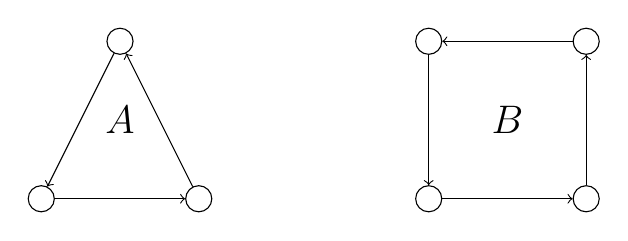
\begin{tikzpicture}[every node/.style={draw,circle}, baseline=(current bounding box.north)]
    \begin{scope}[xshift=-70]
    \node[draw=none, font=\Large] {$\str{A}$};
    \path[->]
      (1,-1) node(n1) {}
      (0,1) node(n2) {}
      (-1,-1) node(n3) {}
      (n1) edge (n2)
      (n2) edge (n3)
      (n3) edge (n1);
    \end{scope}

    \node[draw=none, font=\Large] {$\bisimto_{\GF}$};

    \begin{scope}[xshift=70]
    \node[draw=none, font=\Large] {$\str{B}$};
    \path[->]
      (1,-1) node(n1) {}
      (1,1) node(n2) {}
      (-1,1) node(n3) {}
      (-1,-1) node(n4) {}
      (n1) edge (n2)
      (n2) edge (n3)
      (n3) edge (n4)
      (n4) edge (n1);
    \end{scope}
  \end{tikzpicture}
  \end{figure}
  By design we clearly have $\str{A}\models \phi$ and $\str{B} \not\models \phi$. On the other hand, $\str{A}$ and $\str{B}$ are $\GF$-bisimilar.
\end{example}

Now a similar characterisation can be provided for $\FGF$. 
Due to the ``forwardness'' of the underlying logic, it is convenient to think about maps as tuples.
A \emph{system of forward partial maps} between $\sigma$-structures $\str{A}$ and $\str{B}$ is any non-empty subset of $\bigcup_{i=1}^{\infty} (A^i \times B^i)$ satisfying:
\begin{description}\itemsep0em
  \item[\desclabel{(AtomicEq)}{bisim:atomiceq}] For all $(\elemtuplea, \elemtupleb) \in \bisimZ$ we have that $\elemtuplea$, $\elemtupleb$ are $\sigma$-live and $\tp{\FGF[\sigma]}{\str{A}}{\elemtuplea} = \tp{\FGF[\sigma]}{\str{B}}{\elemtupleb}$~holds.
\end{description}
If $\bisimZ, \bisimZ'$ are systems of forward partial maps between $\str{A}$ and $\str{B}$, we say that $\bisimZ'$ satisfies back-and-forth conditions for $\bisimZ$ if for every $(\elemtuplea, \elemtupleb) \in \bisimZ$ the following conditions hold:
\begin{description}\itemsep0em
  \item[\desclabel{(fForth)}{bisim:fforth}] For every (possibly empty) infix $\elemtuplecfromto{i}{j}$ of $\elemtuplec$ and a $\sigma$-live tuple $\elemtuplee$ in $\str{A}$ such that $\elemtuplecfromto{i}{j} = \elemtupleefromto{1}{j{-}i{+}1}$ there is a $\sigma$-live tuple $\elemtuplef$ with $\elemtupledfromto{i}{j} = \elemtupleffromto{1}{j{-}i{+}1}$ such that $(\elemtuplee, \elemtuplef) \in \bisimZ'$ holds.
  %
  \item[\desclabel{(fBack)}{bisim:fback}] For every (possibly empty) infix $\elemtupledfromto{i}{j}$ of $\elemtupled$ and a $\sigma$-live tuple $\elemtuplef$ in $\str{B}$ such that $\elemtupledfromto{i}{j} = \elemtupleffromto{1}{j{-}i{+}1}$ there is a $\sigma$-live tuple $\elemtuplee$ with $\elemtuplecfromto{i}{j} = \elemtupleefromto{1}{j{-}i{+}1}$ such that $(\elemtuplee, \elemtuplef) \in \bisimZ'$~holds.
\end{description}
A system of forward partial maps $\bisimZ$ between $\str{A}$ and $\str{B}$ is a $\FGF[\sigma]$-\emph{bisimulation} between $\str{A}$ and $\str{B}$ if it itself satisfies the above conditions.\bbeside{Say something that bisimulations are global due to the possibility of empty infix.}
An $\ell$-$\FGF[\sigma]$-bisimulation between $\str{A}$ and $\str{B}$ is a sequence $\bisimZ_0, \bisimZ_1, \ldots, \bisimZ_\ell$ of systems of forward partial maps between $\str{A}$ and $\str{B}$ such that for all $i < \ell$ we have that $\bisimZ_i$ satisfies~\ref{bisim:fforth} and~\ref{bisim:fback} conditions for $\bisimZ_{i{+}1}$.
We speak about $\FGF[\sigma]$-\emph{bisimilar} and $\ell$-$\FGF[\sigma]$-\emph{bisimilar} (pointed) structures in total analogy to the guarded-fragment case.
A ``forward'' counterpart of \cref{lemma:GF-bisimulations-work-well} is presented below.
\begin{lemma}\label{lemma:FGF-bisimulations-work-well}
For every finite signature $\sigma$ and a pair of pointed $\sigma$-structures $(\str{A}, \elemtuplea)$ and~$(\str{B}, \elemtupleb)$ we have that:
\begin{enumerate}[(a)]
\item $(\str{A}, \elemtuplea) \bisimto_{\FGF[\sigma]} (\str{B}, \elemtupleb)$ implies $(\str{A}, \elemtuplea) \equiv_{\FGF[\sigma]} (\str{B}, \elemtupleb)$;
\item $(\str{A}, \elemtuplea) \bisimto_{\FGF[\sigma]}^{\ell} (\str{B}, \elemtupleb)$ implies $(\str{A}, \elemtuplea) \equiv_{\FGF_\ell[\sigma]} (\str{B}, \elemtupleb)$ for all $\ell \in \N$;
\end{enumerate}
Moreover, the converse holds for $\omega$-saturated $\str{A}$ and $\str{B}$.
\end{lemma}
../../Lipics version/proofs/FGF-bisimulations-work-well.tex

The following example presents two structures that are $\FGF$-bisimilar but not $\GF$-bisimilar.
\begin{example} 
Consider a binary predicate $\relE$.
Let $\str{A}$ be a single-element, in which all $\relE$ is interpreted as the full relation, and let $\str{B}$ be an $\relE$-cycle of length two. These two structures are $\FGF[\{\relE\}]$-bisimilar, while a $\GF$-sentence $\exists{\varx_1}\relE(\varx_1,\varx_1)$ can distinguish them.
\end{example}
